\documentclass[tikz,border=2pt]{standalone}
\usetikzlibrary{arrows.meta}
\definecolor{cA}{HTML}{64CADE}\definecolor{cB}{HTML}{6DD2E7}\definecolor{cC}{HTML}{95E1F1}
\definecolor{kA}{HTML}{F19381}\definecolor{kB}{HTML}{FFB1A1}\definecolor{tealD}{HTML}{1F7F92}
\begin{document}
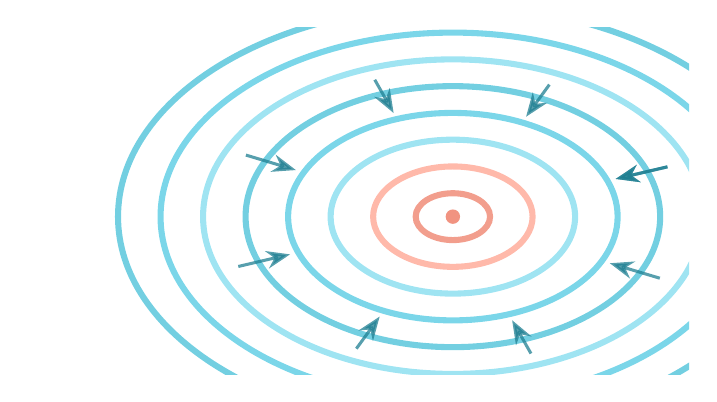
\begin{tikzpicture}
  \clip (-4.2,-2.2) rectangle (4.2,2.2);
  \foreach \r/\c in {0.35/kA,0.75/kB,1.15/cC,1.55/cB,1.95/cA,2.35/cC,2.75/cB,3.15/cA}
     \draw[\c, line width=2.2pt, opacity=.9] (1.2,-.2) ellipse ({1.35*\r} and {0.85*\r});
  \foreach \a in {20,65,...,380}
     \draw[-{Stealth[length=3mm]}, tealD, line width=1.1pt, opacity=.75]
        ({1.2+2.9*cos(\a)},{-.2+1.85*sin(\a)}) -- ({1.2+2.2*cos(\a)},{-.2+1.4*sin(\a)});
  \fill[white] (1.2,-.2) circle (4pt); \fill[kA] (1.2,-.2) circle (2.6pt);
\end{tikzpicture}
\end{document}
